%
% Curriculum Vitæ/Résumé
% Nicolas Dubois <nicolas.c.dubois@gmail.com>
% https://nicolasdubois.com • @wo0dyn
%
% KOMA-Script: scrartcl
%
% This work is licensed under the Creative Commons Attribution-NonCommercial 4.0
% International License.
% To view a copy of this license, visit http://creativecommons.org/licenses/by-nc/4.0/.
%

\documentclass[a4paper, 10pt]{scrartcl}

\usepackage[american, french]{babel}
\usepackage[utf8]{inputenc}
\usepackage[pdftex]{xcolor}

\usepackage{aeguill}
\usepackage{fontawesome}
\usepackage{graphicx}
\usepackage{url}
\usepackage{vmargin}
\usepackage{xifthen}

\usepackage[
  backend=bibtex,
  sorting=ydnt,   % Sort by year (descending), name, title
  style=numeric,  % numeric
]{biblatex}

\usepackage[pdftex, colorlinks,
  pdfpagelayout=SinglePage,
  pdftitle={Curriculum Vitæ},
  pdfauthor={Nicolas Dubois, @wo0dyn},
  pagebackref=false,
  pdfnewwindow=true,
  bookmarksnumbered=true,
  pdfstartview={FitH},
  urlcolor=black,
  linkcolor=black,
]{hyperref}

\bibliography{publications-fr.bib}
\urlstyle{sf}
\pagestyle{empty}
\setmarginsrb
  {10mm} % left margin
  {10mm} % top margin
  {10mm} % right margin
  {10mm} % bottom margin
  {00mm} % head height
  {00mm} % head sep
  {00mm} % foot height
  {00mm} % foot skip

% Refine sections:
\let\customsection\section
  \renewcommand{\section}[1]{
  \addcontentsline{toc}{section}{#1}
  \customsection*{#1 \hrulefill}
}

% Redefine subsections:
\let\customsubsection\subsection
  \renewcommand{\subsection}[1]{
  \addcontentsline{toc}{subsection}{#1}
  \customsubsection*{\hspace{5mm}› #1}
}

% Redefine items:
\let\customitem\item
  \renewcommand{\item}[1]{
  \customitem {\titlefont #1}
}

\definecolor{job-color}{gray}{0.4}

% Custom commands:
\newcommand{\job}[8]{
  % 1: Title
  % 2: Company
  % 3: Location
  % 4: Contrat
  % 5: Started on
  % 6: Finished on
  % 7: Duration
  % 8: Description
  \item{#1}\\
    \faInstitution{} #2 – #4\\
  \textcolor{job-color}{
    \faCalendar{} \ifthenelse{\isempty{#7}}    % if
      {#5 – #6}                                % then
      {#5 – #6 · #7}                           % else
    \\\faMapMarker{} #3
  }
  \ifthenelse{\isempty{#8}}                    % if
    {}                                         % then
    {\begin{quote}\hspace{-7mm}#8\end{quote}}  % else
}
\renewcommand*{\bibfont}{\normalfont\normalsize\sffamily}

\begin{document}

\sffamily

\begin{center}
  {\titlefont\Huge Nicolas Dubois}\\\vspace*{2mm}
  {\titlefont\large Senior Software Engineer (Python/UI)}

  \vspace*{7mm}
  \begin{minipage}[rc]{62mm}
  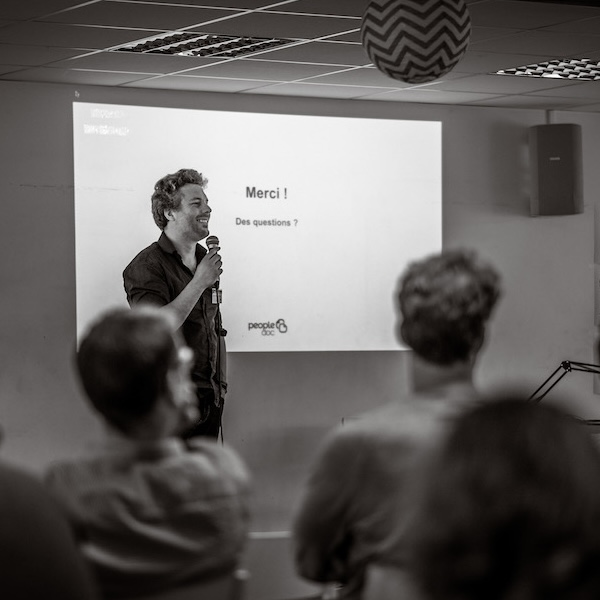
\includegraphics[width=60mm]{images/wo0dyn-at-djangocong-2018-squared.jpg}
  \end{minipage}
  \begin{minipage}{0.6\textwidth}
    \begin{tabular}{p{48mm}@{ }p{85mm}}
      {\bfseries Adresse}\dotfill&
        194 Route de Labrunette\\&
        46110 Bétaille en Quercy\\&
        France\\
      {\bfseries Téléphone}\dotfill&
        \href{tel:+33615316404}{+336 15 31 64 04}\\
      {\bfseries Courriel}\dotfill&
        \href{mailto:nicolas.c.dubois@gmail.com}{nicolas.c.dubois@gmail.com}\\
      \vspace*{1mm}&\vspace*{1mm}\\
      {\bfseries Date de naissance}\dotfill&
        15 juin 1979 à Nancy (54)\\
      {\bfseries Centres d'intérêts}\dotfill&
        Musique (guitare), basketball\\
      \vspace*{1mm}&\vspace*{1mm}\\
      {\bfseries Page personnelle}\dotfill&
        \href{https://nicolasdubois.com}{nicolasdubois.com}\\
      {\bfseries GitHub}\dotfill&
        \href{https://github.com/wo0dyn}{github.com/wo0dyn}\\
      {\bfseries LinkedIn}\dotfill&
        \href{https://www.linkedin.com/in/wo0dyn/}{linkedin.com/in/wo0dyn/}\\
    \end{tabular}
  \end{minipage}


\end{center}

\section{Expérience professionnelle}

\begin{description}
  \job{Senior Software Engineer (Python)}
      {Alma}
      {Télétravail, Paris (75)}
      {CDI}
      {Juin 2021}{Présent}{}{
      Développements sur la plateforme Buy Now–Pay Later (BNPL) d'Alma (API/Dashboard) :
      \begin{list}{•}{}
        \item{Onboarding} Développement d'APIs Hypermédia pour l'onboarding des marchands
        \item{Intl.} Internationalisation/localisation des apps Alma
        \item{API} Développements spécifiques pour l'intégration d'Apple
      \end{list}
  }
  \job{Senior UI Developer (Python), DesignOps Engineer}
      {PeopleDoc/UKG\footnote{\sffamily L'entreprise Ultimate Kronos Group (UKG)
      est issue de la fusion d'Ultimate Software (qui a acquis PeopleDoc
      en 2018) et de Kronos Incorporated.}}
      {Télétravail, Weston, FL \& Lowell, MA, États-Unis d'Amérique}
      {CDI}
      {Mars 2016}{Juin 2021}{5 ans, 4 mois}{
      Développements sur la plateforme de PeopleDoc, avec plusieurs missions :
      \begin{list}{•}{}
        \item{UX/UI} Référent sur les projets Django
        \item{Jinja} Gestion de la migration vers un nouveau Design Language
          System (DLS) dans les templates
        \item{Dashboard} Mise en place des outils de suivi de l'adoption des
          différents composants
        \item{Prototypes} Prototypage de plusieurs applications ayant donné lieu
          à des projets
      \end{list}
  }
  \job{Full Stack Developer (Python)}
      {Oscaro}
      {Télétravail, Gennevilliers (91)}
      {CDI}
      {Avril 2014}{Fév. 2016}{1 an, 11 mois}{
      Développement du site international d'Oscaro sur une stack Linux,
      Python (Django), PostgreSQL, Redis, ElasticSearch.
  }
  \job{Full Stack Developer, Tech Lead}
      {AMG Développement (Groupe GPdis)}
      {Toulouse/Eurocentre (31)}
      {CDI}
      {Octobre 2009}{Avril 2014}{4 ans, 7 mois}{
      Développement d'applications internes de gestion de prix et
      clients (Django) et interventions sur la plateforme Magento du
      groupe (Villatech, Pulsat).
  }
  \job{Web Developer | Project Manager}
      {Ekinos (Groupe Eklas)}
      {Toulouse (31)}
      {CDI}
      {Avril 2009}{Octobre 2009}{7 mois}{
      Développement de boutique en ligne avec la plateforme Magento.
  }
  \job{Full Stack Developer (PHP/symfony)}
      {WaterProof}
      {Montauban (82)}
      {CDI}
      {Novembre 2007}{Avril 2009}{1 an, 6 mois}{
      fdlskfjlsd jflsdkj lfkjsdl kfjlskjl
  }
  % \job{Full Stack Developer (PHP)}
  %     {MaisMoinsCher.com}
  %     {Gaillac (81)}
  %     {CDI}
  %     {Novembre 2005}{Octobre 2007}{2 ans}{
  % }
  % \job{Junior Developer}
  %     {Laboratoire Leibniz (IMAG)}
  %     {Grenoble (38)}
  %     {Stage Master de Recherche}
  %     {Février 2005}{Juillet 2005}{7 mois}{
  % }
\end{description}

\subsection{Conférences}

\begin{quote}
\nocite{*}
\defbibnote{note}{\emph{
  J'ai assisté à de nombreuses conférences au fil des ans et j'ai également
  donné quelques conférences sur le langage Python et son écosystème :}}
\printbibliography[heading=none,prenote=note,type=inproceedings]
\end{quote}

\subsection{Enseignement}

\begin{description}
  \job{Web Developer/Designer}
      {Vidéoscop de Nancy}
      {Nancy (54)}
      {Vacation}
      {Mars 2003}{Juin 2003}{4 mois}{
      Médiatisation du cours d'Interface Homme-Machine (IHM) de Pr.~Kamel
      Smaïli (Université de Lorraine) pour le projet e-miage.
  }
  \job{Tuteur}
      {Université Nancy 2}
      {Nancy (54)}
      {Tuteur}
      {Février 2002}{Juin 2002}{5 mois}{
      Tuteur en informatique à la faculté d'AES : initiation aux outils
      de bureautique.
  }
\end{description}

\section{Formation}

\begin{description}
    \item{2004 – 2005 : Master 2 de Recherche (DEA) "Information,
      Cognition et Apprentissages"}, spécialité Sciences Cognitives
      \begin{quote}\faBook{} \fullcite{masterthesis2005}\end{quote}
    \item{2003 – 2004 : Maîtrise de Sciences Cognitives}
      \begin{quote}\faBook{} \fullcite{ter2004}\end{quote}
    \item{2002 – 2003 : Licence de Sciences Cognitives} obtenue à l'Université Nancy 2
\end{description}

\section{Savoir-faire}

% \subsection{Techniques}

\begin{description}
  \item{Environnements : }\textbf{macOS}, \textbf{GNU/Linux} (Debian/Ubuntu) ;
  \item{Langages : }\textbf{Python}, Unix Shells (bash/zsh), {\LaTeX} ;
  \item{Développement Web : }\textbf{HTML5}, \textbf{CSS3}, JavaScript, htmx ;
  \item{Bases de Données : }\textbf{PostgreSQL}, SQLite ;
  \item{Frameworks : }\textbf{FastAPI}, \textbf{Django} et flask.
  \item{Notions : }ElasticSearch, Java, Redis, React.js/TypeScript, PHP, MySQL, XML/XSL.
\end{description}

\subsection{Langues}

\textbf{Français : }langue maternelle •
\textbf{Anglais : }lu, écrit, parlé (B2{\scriptsize +}) •
\textbf{Espagnol : }notions (A1)

\end{document}
